81. \begin{figure}[ht!]
\center{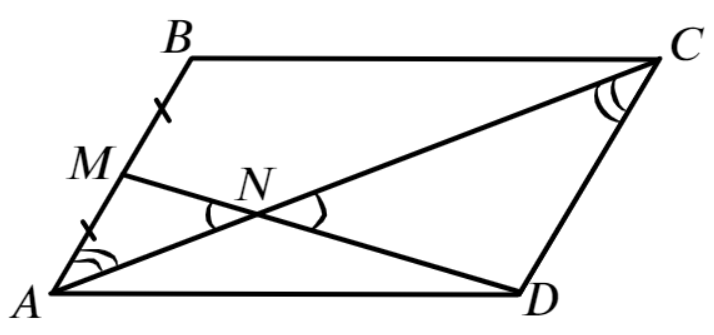
\includegraphics[scale=0.35]{g8-80.png}}
\end{figure}\\
Треугольники $AMN$ и $CND$ подобны по двум углам ($MNA$ и $CND$ вертикальные, $MAN$ и $NCD$ накрест лежащие), поэтому $\cfrac{NC}{NA}=\cfrac{CD}{AM}=\cfrac{AB}{AM}=2,$ значит $NC=2NA$ и $NC+NA=15,$ откуда $NA=5,\ NC=10.$\\
